% !TeX root = ../Document.tex
\documentclass[../Document.tex]{subfiles}

\begin{document}
\section{Koračni motori}
Koračni motori su tip DC elektronskog motora bez četkica. Revoluciju dijele u jednake korake odakle i dolazi njihov naziv. Ovi motori zbog toga mogu biti precizno pomjereni i zadržani na željenoj poziciji bez enkodera pozicije.
\vspace{0.5cm}
\subsection{Elektromagneti}
Elektromagneti su tipovi magneta koji svoja magneta svojstva pokazuju kada kroz njih teče elktrična struja. Jedno od svojstava protoka struje kroz provodnik je magnetno polje koje se stvara oko provodnika. Ovo svojstvo se može multiplicirati zavijanjem izoliranog provodnika u spiralu oko provodničkog jezgra. Za razliku od trajnih magneta, magnetna svojstva ovih uređaja mogu biti aktivirana po potrebi.\\

\begin{figure}[h]
    \centering
    \hspace{1.8cm}
    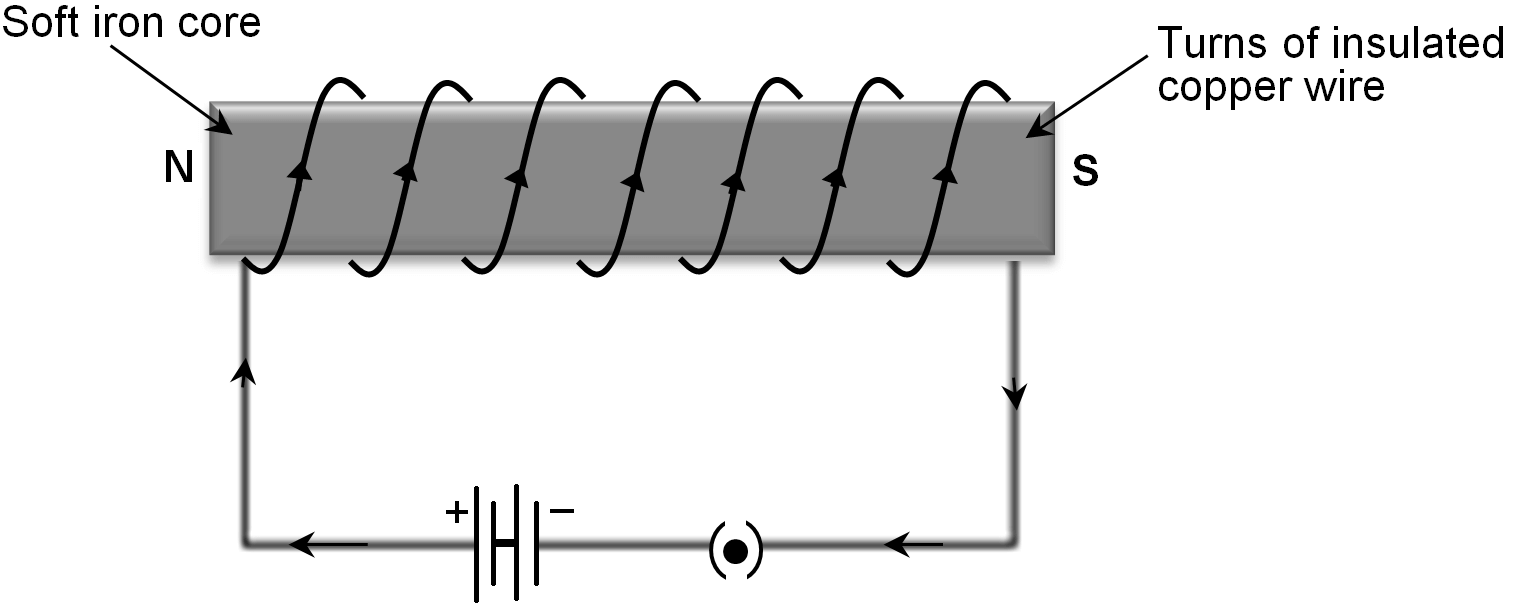
\includegraphics[width=0.8\textwidth]{Stepper-Motor_Elektromagnet}
    \caption{Elektromagnet}
\end{figure}

\subsection{Proces rotacije osovine}
Koračni motori su građeni iz okvira (koji čine elektromagneti) i jezgra - željeznog zupčanika koji je ujedno i trajni magnet. Ovi magneti su najčešće kontrolisani od strane mikrokontrolera ili upravljača koji nije dio samog motora. Do rotacije osovine motora dolazi puštanjem električne struje kroz jedan elektromagnet. Nakon što se povučen magnetnom silom zupčanik fiksira na poziciju, paljenjem drugog elektromagneta postiže se rotacija ose motora na željenu poziciju. Ova rotacija predstavlja koncept koraka gdje prirodni broj N koraka čini jednu revoluciju osovine motora.

\subsection{Tipovi}
Postoje dva tipa koračnih motora:

\subparagraph{Uniopolarni} \noindent imaju elektromagnete sa središnjim izlazom (eng. center tap). To omogućava da promjenom kraja na kojem je uzemljenje elektromotora, samo polovina elektromagneta bude magnetizirana.\\

\cFigure{Stepper-Motor_Unipolarni}{Šema unipolarnog motora}{0.35}

\subparagraph{Bipolarni} \noindent koračni motori imaju samo po jednu žicu na oba kraja elektrom od kojih je jedna spojena na uzemljenje, a druga na izvor struje. Ovo omogućava jače magnetno djelovanje, kao i kreiranje magnetnog polja u oba smijera na zajedničkom prostoru.\\

\cFigure{Stepper-Motor_Bipolarni}{Šema bipolarnog motora}{0.35}

\noindent Prednost bipolarnih motora je veća vučna sila i jače magnetno polje, a kod unipolarnih su to manji troškovi zbog jednostavnije kontrole, kao i manji otpor\cite{unipolarvsbipolar}.

\subsection{Načini upravljanja}
U praksi postoje 4 načina upravljanja koračnim motorima

\subparagraph{Valno upravljanje} je metoda gdje se u jednom trenutku šalje samo jedna faza. Ovo upravljanje se rijetko koristi jer ima jednak broj koraka kao upravljanje punim korakom, ali samo 50\% njegove vučne sile. Ukoliko zupčanik ra rotoru ima 25 zuba, onda će se svaki taj zub pomjeriti pomoću 4 faze. To znači da će se sa 100 koraka napraviti jedna revolucija.\\
\cFigure{Stepper-Motor_Valni}{Valno upravljanje}{1}

\subparagraph{Metoda punog koraka} je najčešće korištena metoda upravljanja. U svakom trenutku ima tačno dvije faze. Ovom metodom se izvlači maksimalna vučna sila motora, dok također ima 100 koraka po revoluciji.\\
\cFigure{Stepper-Motor_Puni-Korak}{Metoda punog koraka}{1}


\subparagraph{Polukoračno} upravljanje se svodi na promjenu dvije faze za vrijeme jedne. Ovo motoru smanjuje vučnu silu, ali udvostručava rezoluciju. Kako je sada potrebno 8 faza kako bi se zupčanik pomjerio za jedan zub, jedna  revolucija zahtjeva 200 koraka.\\
\cFigure{Stepper-Motor_Polukorak}{Polukoračno upravljanje}{1}


\subparagraph{Mikrokoračanje} je metoda u kojoj se sinusnom i kosinusnom funkcijom kreiraju faze. Ovo znatno smanjuje broj koraka u jednoj revoluciji, čime se povećava rezolucija samog motora. U ovim situacijama, ograničenje broja koraka u revoluciji postoji zbog statičkog trenja i zazora.\\
\cFigure{Stepper-Motor_Mikrokorak}{Mikrokoračanje}{1}

\noindent Kako bi se postigle veće brzine kretanja motora, potrebna je akceleracija koja će motor dovesti do pune brzine. U primjeni sam također zapazio da se deakceleracijom pri promjeni smjera postiže bolji rezultat kod promjene smjera kretanja.

\end{document}